\frame{
  \frametitle{Decision Trees}
  \begin{columns}
    \begin{column}{0.5\textwidth}
    \begin{itemize}
        \item Each node represents a query, each leaf represents a category/decision.

        \medskip
        
        \item Commonly used in decision analysis and machine learning 

        \medskip

        \item Fuzzy Decision Trees are also a thing
    \end{itemize}
    \end{column}
    \begin{column}{0.5\textwidth}  %%<--- here
        \begin{center}
            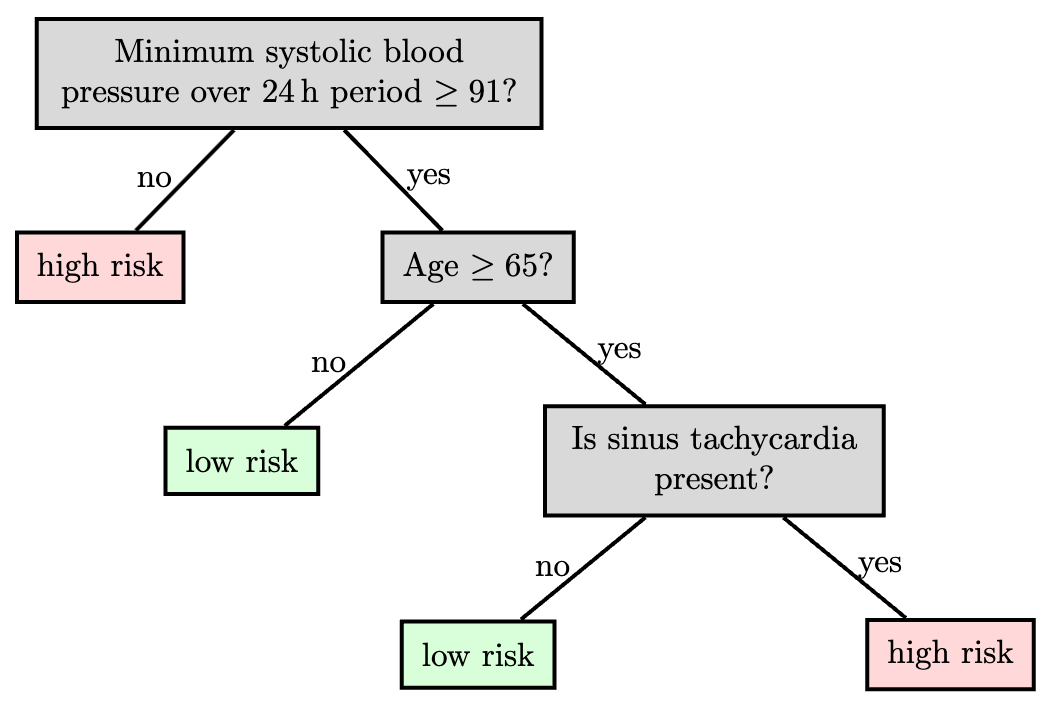
\includegraphics[scale=0.4]{slides/alphabet_trees/decision_tree.png} % TODO : change this to something way funnier

            {\tiny MIT 6.390 Intro ML Course Notes and Breiman, Friedman, Olshen, Stone (1984)}
         \end{center}
    \end{column}
    \end{columns}
}

\frame{
  \frametitle{(Furry) Decision Trees (\texttt{r/furry/comments/4gxm0l/})}
    \begin{center}
        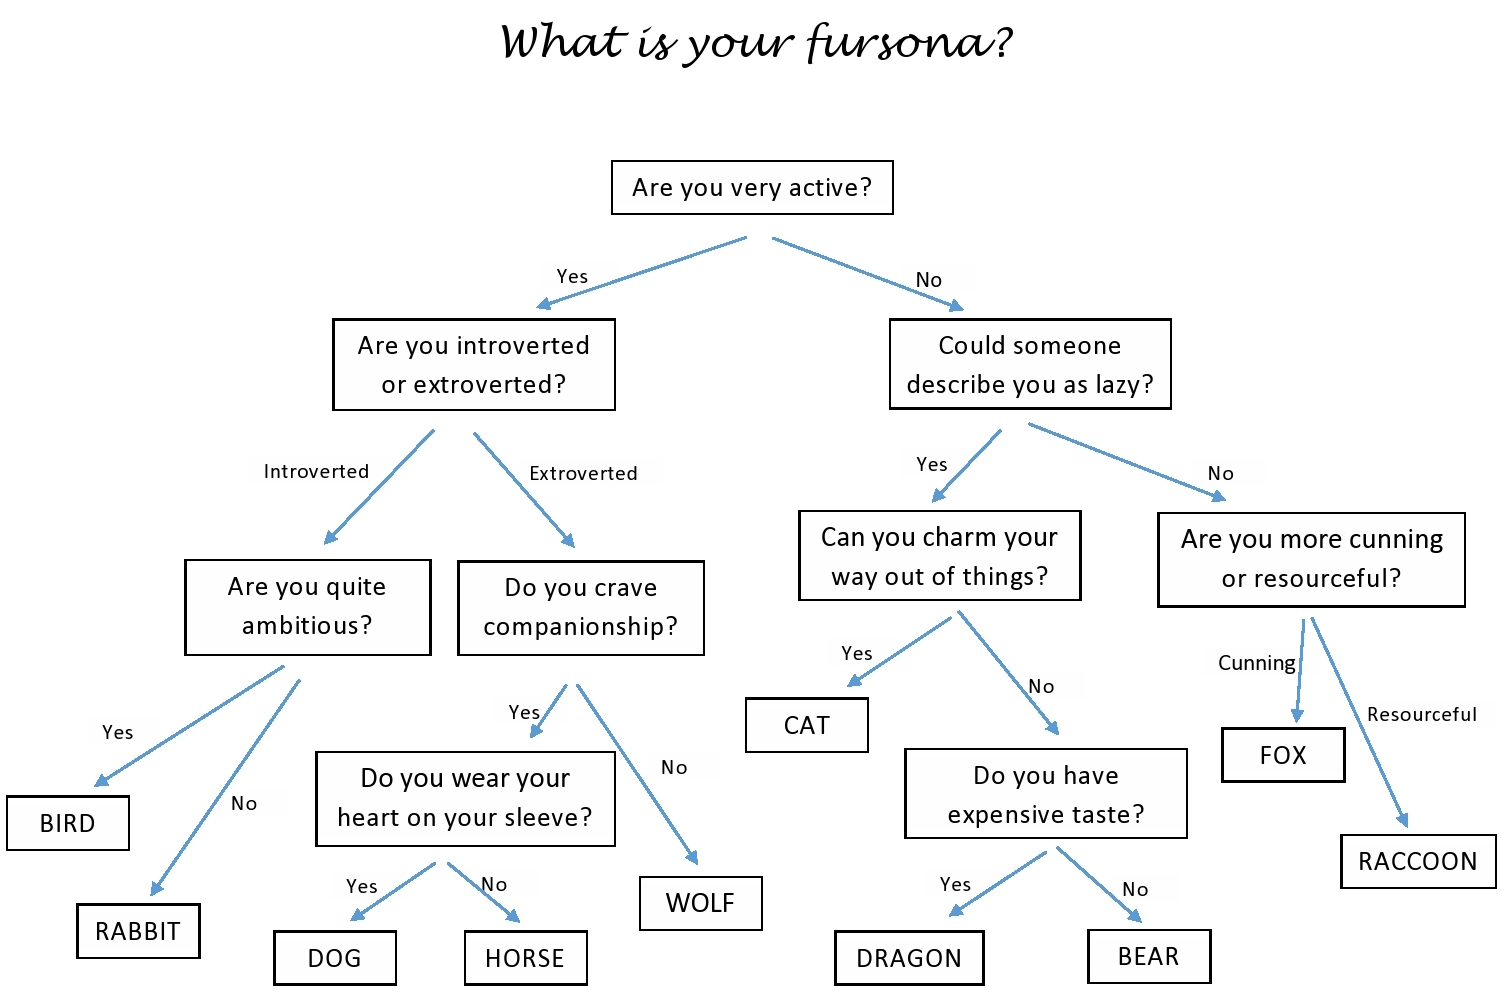
\includegraphics[scale=0.25]{slides/alphabet_trees/furry_decision_tree.jpeg}
    
    {\tiny }
        
     \end{center}
}
